\documentclass[10pt,a4paper]{article}
\usepackage[margin=2.2cm]{geometry}
\usepackage{fontspec}
\usepackage{kotex}
\setmainfont{Apple SD Gothic Neo}
\setsansfont{Apple SD Gothic Neo}
\usepackage{amsmath,amssymb}
\usepackage{graphicx}
\usepackage{booktabs}
\usepackage{caption}
\usepackage[dvipsnames]{xcolor}
\usepackage[colorlinks=true,linkcolor=MidnightBlue,citecolor=MidnightBlue,
            urlcolor=MidnightBlue]{hyperref}
\usepackage{titlesec}
\titleformat{\section}{\large\bfseries}{\thesection}{0.6em}{}
\titleformat{\subsection}{\normalsize\bfseries}{\thesubsection}{0.5em}{}
\captionsetup{font=small,labelfont=bf}
\setlength{\parskip}{0.35em}
\setlength{\parindent}{0pt}

\usepackage{mdframed}
\newmdenv[linewidth=0.4pt,linecolor=gray!60,backgroundcolor=gray!5,
          innertopmargin=6pt,innerbottommargin=6pt,skipabove=8pt,skipbelow=8pt]{claimbox}
\newcommand{\claim}[2]{\begin{claimbox}\textbf{주장.} #1\par\smallskip
  \textcolor{gray!70}{\textbf{반증 조건.} #2}\end{claimbox}}

\title{\bfseries $1.6\sigma$ 와 $6.2\sigma$\\[2pt]
\large 같은 ``$2\sigma$'' 라고 적힌 문턱을 참값 $0$ 으로 재니 짝마다 네 배 어긋나 있었다}
\author{월드모델 실험실 · 노트 714 · 715}
\date{2026-08-06}
\begin{document}\maketitle

\section{한 줄}

채택 문턱을 \textbf{위약 대 위약}으로 쟀다 --- 참값이 $0$ 인 두 팔의 차. 기록된
문턱이 \textbf{앱에서 $1.6\sigma$}(오탐률 $27.8\%$)이고 \textbf{KR 만화에서
$6.2\sigma$}(실제 신호를 놓친다)다. \textbf{행수로 설명되지 않는다} --- 두 짝이
$1{,}600$과 $1{,}716$행인데 참값 $0$ 차의 SD 가 네 배 다르다.

\section{왜 이것을 쟀나 --- 규약에 구멍이 있었다}

규약 아홉이 \emph{``규약이 요구하는 다섯 자''}를 말하는데 \textbf{몇 개가
통과해야 채택인지는 대장 어디에도 없었다.} 그리고 지금 상태가 하필 갈리는
자리다 --- 둘 통과(판 $2.6$배 · 앱 $3.5$배) 둘 미달(CN · KR).

\textbf{이 상태를 보고 규칙을 정하면 그것이 체리피킹이다.} ``과반''이라 하면
채택되고 ``전부''라 하면 보류된다. 그래서 \textbf{결과와 독립적인 근거로
도출}하고 그 도출을 측정으로 검증했다.

\subsection*{도출 --- 계산에서 나온다}

자 여섯은 두 갈래다. \textbf{집안 셋}(판 · 날짜 통제 판 · 무리 안 판 --- 같은
$3{,}369$행)과 \textbf{집 밖 셋}(KR · CN 만화 · 비게임 앱 --- 판이 한 줄도 학습하지
않은 행). \textbf{둘은 다른 물음이라 대체할 수 없다} --- 집안은 ``이 판이
좋아졌나'', 집 밖은 ``옮겨 가나''.

그리고 노트 629 가 \textbf{집 밖 세 짝이 거의 완전 독립}($2.99/3$)임을 쟀다.
각 문턱이 $2\sigma$($\approx 5\%$)이고 독립이면 우연히 넘는 확률은
$\ge 1$ 이 $14\%$ · $\ge 2$ 가 $0.7\%$ · $\ge 3$ 이 $0.01\%$ 다. 도출되는 규칙:

\begin{center}\textbf{집안 $\ge 1$ 이고 집 밖 $\ge 2$}\end{center}

\textbf{이 규칙을 결과 보기 전에 사전등록했다}(노트 714). 그리고 그 계산이 가정한
\emph{``문턱이 $5\%$ 를 가른다''}를 검증한 것이 이 논문이다.

\section{위약 대 위약 --- 참값이 0 인 자}

같은 판에서 \textbf{독립적인 위약 셔플 넷}을 만들고 그 쌍들의 ``신호 몫''을 냈다.
참값은 $0$ 이므로, 그 분포가 문턱을 넘는 비율이 \textbf{실제 오탐률}이다.
배선은 비싼 쪽을 공유한다 --- \textbf{씨앗마다 판을 한 번만 적합하고} 짝 셋 ×
위약 넷을 그 위에서 예측한다(짝마다 따로 적합하면 여섯 배 든다).

\begin{figure}[t]\centering
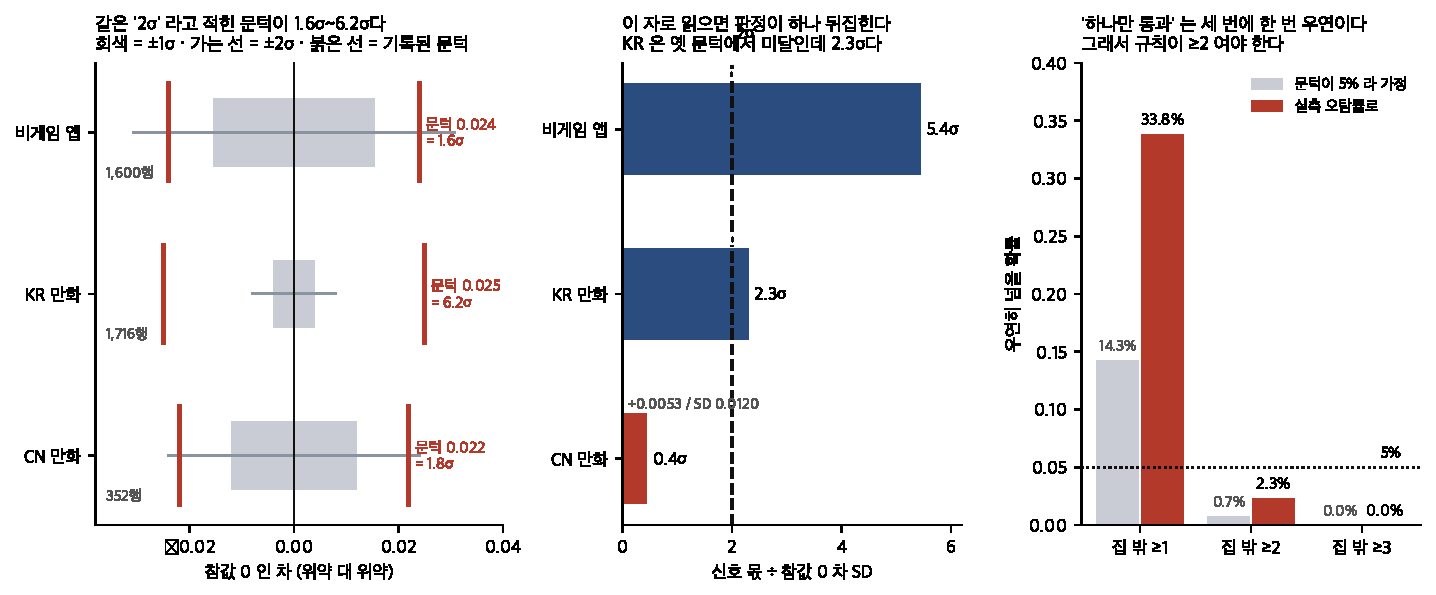
\includegraphics[width=0.99\textwidth]{figs/sigma.pdf}
\caption{왼쪽: 참값 $0$ 분포와 기록된 문턱. \textbf{같은 ``$2\sigma$''가 실제로는
$1.6$--$6.2\sigma$다.} 가운데: 그 자로 읽은 신호. \textbf{KR 이 옛 문턱에서
미달인데 $2.3\sigma$다.} 오른쪽: ``집 밖 $\ge k$''의 우연 확률 --- 가정 대 실측.}
\end{figure}

\begin{center}
\begin{tabular}{lrrrrr}
\toprule
짝 & 행 & 문턱 & 참값 $0$ 차 SD & \textbf{문턱이 몇 $\sigma$} & 오탐률 \\
\midrule
비게임 앱 & $1{,}600$ & $0.024$ & $\mathbf{0.0154}$ & $\mathbf{1.6\sigma}$ & $\mathbf{27.8\%}$ \\
KR 만화 & $1{,}716$ & $0.025$ & $\mathbf{0.0040}$ & $\mathbf{6.2\sigma}$ & $0.0\%$ \\
CN 만화 & $352$ & $0.022$ & $0.0120$ & $1.8\sigma$ & $8.3\%$ \\
\midrule
\multicolumn{5}{l}{전체 (위약 쌍 18개 중 2개가 문턱 밖)} & $\mathbf{11.1\%}$ \\
\bottomrule
\end{tabular}
\end{center}

사전등록 예측은 \emph{``오탐률이 $5\%$ 보다 클 것 --- $8$--$20\%$''} 였고
$11.1\%$ 로 \textbf{맞았다}. 근거도 맞았다 --- 문턱은 노트 583/586 때 잡은 값이고
그 뒤 자료가 자랐다.

\claim{\textbf{``$2\sigma$'' 라고 적힌 문턱이 실제로 몇 $\sigma$ 인지는 짝마다
다르고, 어긋나는 \emph{방향}도 다르다.} 앱에서는 너무 낮아 $27.8\%$ 를 통과시키고
KR 에서는 너무 높아 실제 신호를 놓친다. \textbf{그러므로 문턱을 인용할 때 그것이
몇 $\sigma$ 인지 같이 적어야 한다.}}
{참값 $0$ 차 SD 를 씨앗 6 · 위약 4 로 쟀다. 위약 8 · 씨앗 12 로 늘렸을 때 SD 가
크게 달라지면 이 표가 흔들린다 --- 특히 KR 의 $0.0040$ 은 작아서 표본에 민감할
수 있다.}

\subsection*{행수로 설명되지 않는다}

앱 $1{,}600$행과 KR $1{,}716$행은 거의 같은데 참값 $0$ 차 SD 가 $0.0154$ 대
$0.0040$ 으로 \textbf{네 배}다. 노트 712 는 CN($352$행)이 씨앗 3 에서 안정되지
않은 것을 \emph{행수}로 설명했는데 \textbf{그 설명이 여기서는 안 통한다.}

\claim{\textbf{짝의 잡음 크기는 행수가 아니라 다른 것이 정한다.} 후보 둘 ---
\textbf{라벨 분포}(노트 691 이 라벨 자리폭을 짝마다 쟀다)와 \textbf{텍스트 예보의
퍼짐}(노트 712: 앱 $0.158$ 대 KR $0.0967$). 다만 예보 퍼짐은 두 배 차이인데 SD 는
네 배라 그것만으로는 안 맞는다.}
{행수를 통제한 짝 짝(비슷한 행수 · 다른 라벨 분포)을 더 만들어 재면 갈린다.
지금은 $n=3$ 이고 그중 둘이 행수가 비슷하다.}

\section{규칙은 살아남았다 --- 그리고 더 필요해졌다}

실측 오탐률로 다시 계산하면:

\begin{center}
\begin{tabular}{lrr}
\toprule
 & 문턱이 $5\%$ 라 가정 & \textbf{실측 오탐률로} \\
\midrule
집 밖 $\ge 1$ & $14.3\%$ & $\mathbf{33.8\%}$ \\
집 밖 $\ge 2$ & $0.7\%$ & $\mathbf{2.3\%}$ \\
집 밖 $\ge 3$ & $0.01\%$ & $0.00\%$ \\
\bottomrule
\end{tabular}
\end{center}

\textbf{``집 밖 하나만 통과''는 세 번에 한 번 우연히 일어난다.} 규칙이 필요하다는
것이 훨씬 강하게 확인됐다. 그리고 $\ge 2$ 는 $2.3\%$ 로 $5\%$ 안이므로
\textbf{도출한 규칙은 그대로 선다}(다만 계산했던 $0.7\%$ 보다 세 배 느슨하다).

\subsection*{독립 확인 --- 노트 710 이 같은 것을 말한다}

CN 의 참값 $0$ 차 절대값 최대가 $\mathbf{0.0214}$ 이고 문턱이 $0.022$ 다. 노트 709
가 씨앗 3 에서 잰 CN 신호 몫 $\mathbf{+0.0271}$ 은 그 바로 위였고, 노트 710 이 씨앗
12 로 $\mathbf{+0.0053}$ 으로 무너뜨렸다. \textbf{두 측정이 서로 모르고 같은 것을
말한다} --- 그 통과는 참값 $0$ 분포의 꼬리였다.

\section{KR 을 지금 통과로 바꾸지 않는다}

새 문턱을 $2 \times$(참값 $0$ 차 SD)로 잡으면 앱 $0.0308$ · KR $\mathbf{0.0080}$ ·
CN $0.0240$ 이다. 그러면 판정이 \textbf{앱 통과 · KR 통과 · CN 미달}이 되어
\textbf{집 밖 $2/3$} 이고 도출한 규칙을 \emph{충족한다}.

\claim{\textbf{그렇게 선언하지 않는다.} 노트 714 사전등록에 \emph{``문턱은 기록된
표본 $2\sigma$ 를 그대로 쓴다 --- 이 실험이 그것을 검증하는 것이므로 바꾸지
않는다''}고 적었다. \textbf{지금 고치면 결과를 보고 규칙을 바꾸는 것이고}, 그것이
노트 133 이 막으려는 바로 그 일이다. 문턱 개정은 \textbf{다음 사이클의 사전등록
대상}이다.}
{사전등록에 그 문장이 없었다면 이 논문에서 개정해도 됐다. 있으므로 안 한다 ---
그 문장의 커밋 시각이 이 측정보다 앞선다는 것이 이 절이 설 수 있는 근거다.}

그리고 개정 전에 셋을 채워야 한다. ① 참값 $0$ SD 를 \textbf{위약 8 · 씨앗 12}로
굳힌다. ② KR 이 $0.0092$ 대 $0.0080$ 으로 \textbf{$1.15$배}인데, 그것은 노트 710
에서 무너진 CN($1.23$배)과 \emph{같은 거리}다. ③ \textbf{왜 짝마다 SD 가 네 배
다른지} 모른다.

\end{document}
